\begin{figure}[t]
  \centering
  \begin{adjustbox}{minipage=\textwidth, scale=0.85}
  \usetikzlibrary{shapes.arrows}
  \definecolor{tile0}{HTML}{DABDE4}
  \definecolor{tile1}{HTML}{B8DBF4}
  \definecolor{tile2}{HTML}{B5EDCD}
  \definecolor{tile3}{HTML}{FBEBA7}
  \definecolor{tile4}{HTML}{F9C1BB}

  \tikzstyle{array_element}=[rectangle,
                           minimum height=1cm, 
                           minimum width=1cm, 
                           minimum size=1cm,
                           draw=black,
                           rounded corners=2.5 ]
  
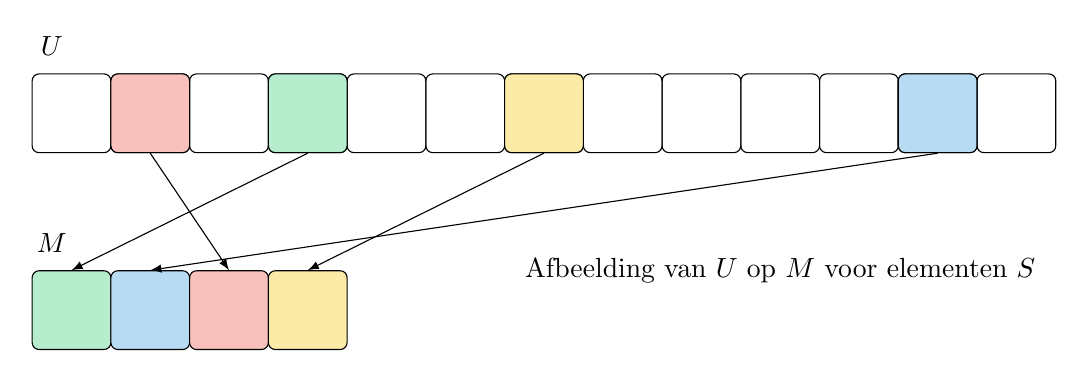
\begin{tikzpicture}
  \foreach \lb in {0,...,12} {
    \node at (1.0cm * \lb, 0.0cm) () [array_element] {};
  }
  \node at (1.0cm, 0.0cm) (U1) [array_element, fill=tile4] {};
  \node at (3.0cm, 0.0cm) (U2) [array_element, fill=tile2] {};
  \node at (6.0cm, 0.0cm) (U3) [array_element, fill=tile3] {};
  \node at (11.0cm, 0.0cm) (U4) [array_element, fill=tile1] {};

  \node at (0.0cm, -2.5cm) (M2) [array_element, fill=tile2] {};
  \node at (1.0cm, -2.5cm) (M4) [array_element, fill=tile1] {};
  \node at (2.0cm, -2.5cm) (M1) [array_element, fill=tile4] {};
  \node at (3.0cm, -2.5cm) (M3) [array_element, fill=tile3] {};

  \draw[-latex] (U1.south) -- (M1.north);
  \draw[-latex] (U2.south) -- (M2.north);
  \draw[-latex] (U3.south) -- (M3.north);
  \draw[-latex] (U4.south) -- (M4.north);

  \node at(-0.25cm, 0.85cm) (U) [] {$U$};
  \node at(-0.25cm, 0.85cm - 2.5cm) (U) [] {$M$};
  \node at(9.0cm, -2.0cm) (U) [] {Afbeelding van $U$ op $M$ voor elementen $S$};
  \end{tikzpicture}
  \end{adjustbox}
  \caption{Afbeelding van $U$ op $M$.}
  \label{fig:hs-hashfunctie}
\end{figure}
